\documentclass[a4paper]{article}
\usepackage{url}
\usepackage{hyperref}
\usepackage{appendix}
\usepackage{xcolor}
\usepackage{graphicx}
\usepackage{float}
\usepackage{multicol}
\usepackage{fancyhdr}
\usepackage{listings}
\usepackage{caption}
\usepackage{amsmath}
\usepackage{report_style}
\usepackage{siunitx}
\sisetup{
  round-mode = places,
  round-precision = 2,
  group-separator = {,},
  group-minimum-digits = 4,
}

\DeclareCaptionFormat{codecaption}{#3} % Remove the prefix and separator
\captionsetup[lstlisting]{format=codecaption} % Apply the custom format to lstlisting captions

% Define custom Python style
\lstdefinestyle{pythoncode}{
    language=Python,
    basicstyle=\ttfamily\footnotesize,
    numbers=left,
    numberstyle=\tiny,
    stepnumber=1,
    numbersep=5pt,
    xleftmargin=15pt,
    showspaces=false,
    showstringspaces=false,
    showtabs=false,
    framextopmargin=5pt,
    framexbottommargin=5pt,
    frame=tb,
    rulecolor=\color{black},
    tabsize=4,
    captionpos=b,
    breaklines=true,
    breakatwhitespace=true,
    title=\lstname,
    commentstyle=\color{white},
}

\title{Pricing European Options with Neural Networks and Gradient Boosted Decision Trees}

\author{
Juan Esteban Berger \\ University of Notre Dame \\ jberger8@nd.edu \\
May 8, 2023
}

\pagestyle{fancy}
\fancyhf{} % clear all header and footer fields
\fancyfoot[C]{\thepage} % center the page number
\renewcommand{\headrulewidth}{0pt} % remove the header rule

\begin{document}
\maketitle

\begin{abstract}
This paper provides a comparison of using Neural Networks and Gradient Boosted Decision Trees for pricing European Options. The Neural Network models were implemented using TensorFlow, and the Gradient Boosted Decision Tree models were implemented using XGBoost. Both the TensorFlow and the XGBoost models can outperform the Black-Scholes Model in terms of Mean Absolute Error and Mean Absolute Percentage Error. These results showcase the potential that using historical data from the underlying asset can have when pricing options, especially when using machine learning algorithms to learn complex features that traditional parametric models may not be able to detect.
\end{abstract}


\section{Introduction}

The XGBoost algorithm has been regarded as the gold standard for machine shortly after its inception in 2014. On the other hand, Neural Networks have showcased incredible abilities in being able to learn extremely complicated functions with large numbers of variables. This study hopes to find out if deep learning algorithms are able to surpass the gold standard machine learning algorithm XGBoost in the problem of options pricing. This study will focus on pricing European Options from the IvyDB US dataset from Option Metrics and the results of various Neural Network Models and various XGBoost models will be compared with the prices derived from the Black-Scholes Model, one of the classical parametric options pricing methodologies.

\section{Related Work}

In 2019, Stanford University students Yang and Ke \cite{ke2019option} studied Long-Short Term Memory Networks and Feed-Forward Neural Networks (referred to as Multilayer Perceptrons in their paper) for the purpose of pricing Options. These students used data sourced from Option Metrics' IvyDB US dataset \cite{optionmetrics}, the same data source used for training the models in this paper. Yang and Ke decide not to use the implied volatility listed in the IvyDB US dataset and to use the closing price over 20 timesteps instead to train their Long Short Term Memory Neural Networks with the hopes that the Neural Networks will be able to learn this information (and many more features) from the past lags of the underlying assets price. However, unlike the Yang and Ke's models, no recurrent neural networks were used in this study, but instead the past 20 daily closing prices for the underlying asset were used as individual features (along with an options strike price, current underlying price, risk-free rate, dividend yield, and whether the option was a call or a put) to train the Feed-Forward Neural Networks used in this study. Finally, Yange and Ke assessed the performance of their models according the Mean Squared Error and Mean Absolute Percentage Error (among other performance metrics). The results of this study show how both standard feed-forward neural networks (i.e. Multi Layer Perceptrons) and Long Short Term Memory networks are able to outperform the Black-Scholes Model in both Mean Squared Error and Mean Absolute Percentage Error.

Furthermore, Neural Networks have been studied for the purposes of pricing options since the early 1990s. In 1993, Malliaris and Salchenberg \cite{malliaris1993beating} implemented Neural Networks that used an Options underlying price, the options' strike price, the time to expiration, the options' implied volatility, the risk free rate, and past lags of the option's price and the underlying asset's price to predict an Options' current price. Even as early as 1993, the results of that study showed how Neural Networks could outperform the Black-Scholes model for both in-the-money and out-the-money options. Another interesting study was performed le Roux and du Toit \cite{leRoux2001}. In this study, an Option's underlying price, strike price, time to maturity, implied volatility and risk-free rate are used to estimate the price of an option. This study showed that Neural Networks were able to emulate the Black-Scholes model with an accuracy of at least 99.5\% with a confidence interval of 96\%. These results are remarkable considering the relatively simple neural network architectures and the lack of computing power in the early 1990s and 2000s.

More modern, studies have been performed focused on pricing options with Neural Networks like those by Mitra in 2012 \cite{mitra2012option} and by Can and Fadda in 2014 \cite{can2014nonparametric}. The study by Mitra used an Option's underlying asset's price, an option's strike price, the time to maturity, the historical volatility of the underlying asset's price, and the risk-free rate in order to predict an Option's price and showed that neural networks could be used to improve theoretical option pricing approaches since they are able to learn features that are hard to incorporate into the classical approaches. Furthermore, Can and Fadda use the a slgihtly different approach to pricing options by using an Option's underlying price divided by its' strike price as one of the features along with the options' underlying price, the time to maturity, and the risk free rate in order to estimate the value of the Option's price divided by the strike price. Once again, Neural Networks are shown to overperform the Black Scholes model in terms of Mean Absolute Error. Finally, a highly thorough literature review was performed in 2020 by Ruf and Wang \cite{ruf2020neural} where they summarize the methods and findings of using Neural Networks for Options Pricing and Hedging since the 1990s up until modern findings from 2019.

\section{Data Sourcing}
The data for this study was sourced from the Option Metrics' IvyDB US dataset. OptionMetrics is a financial research and consulting firm that provides historical options data and analytics on global exchange-traded options. It is a subsidiary of Wharton Research Data Services. The IvyDB US dataset includes many tables with historical market, options, and securities data ranging from 1990 to 2021 (as of this writing). The final dataset used to train the models consisted of 10,750,886 observations. The target variable was the midpoint price (which was calculated as the average between the bid and ask price for a given function. The feature variables were the option's strike price, implied volatility, the zero coupon rate, the index dividend yields, the option type (either call or put), the time to maturity in years, and the underlying assets current price. The past 20 days' closing price were also included as 20 additional feature variables for the dataset. Some filters that were applied to the dataset were that only European Options had indexes as underlying assets. Furthermore, only options with midpoint prices greater than 0.01 and less than 100,000 were selected with the goals of eliminating outliers from the dataset.
Furthermore, big data technologies had to be used for querying and cleaning the data since the original dataset was over 500GB large. In order to efficiently query and the data, Google Cloud Storage and were BigQuery utilized. Finally, the data was split into training, validation, and testing datasets with approximates splits of 98\% of the data being used for training, 1\% of the data being used for validation, and 1\% being used for testing. The code for querying the dataset and additional details about the tables sourced and their sizes can be found through this \href{https://github.com/juan-esteban-berger/Options_Pricing_with_Neural_Networks_and_Gradient_Boosters/blob/main/01_Data_Cleansing.ipynb}{\textcolor{blue}{link.}} The summary statistics of the target and feature variables can be found at figure Please see Table \ref{table:financialdata}. The distributions for all of the target and feature variables can be found at the \hyperref[sec:appendix]{Appendix.}

\section{Modeling}
Six models were implemented with Python for pricing options. These models were the Black-Scholes Model, a 3 Layer Feed-Forward Neural Network, a 4 Layer Feed-Forward Neural Network, a 5 Layer Feed-Forward Neural Network, an Gradient Boosted Decision Tree with a Max Depth of 5 and a Gradient Boosted Decision Tree with a Max Depth of 10. The Feed-Forward Neural Networks were implemented with Tensorflow Framework and trained using distributed training on Google Colab's TPU's (which had 8 devices available). The Gradient Boosted Decision Tree Models were implemented using the XGBoost Framework and trained on Google Colab's A100 GPU. The complete code for all of these models can be found through this \href{https://github.com/juan-esteban-berger/Options_Pricing_with_Neural_Networks_and_Gradient_Boosters/blob/main/03_Modeling.ipynb}{\textcolor{blue}{link.}}
\subsection{Black-Scholes Model}
The Options in the data used for this study were all European Options and can be priced according to the Black-Scholes Model:
$$
C = Se^{-qT}N(d_1)-Ke^{-rT}N(d_2)
$$
$$
P = Ke^{-rT}N(-d_2)-Se^{-qT}N(-d_1)
$$
where
$$
d_1 = [\ln(S/K) + (r - q + \tfrac{1}{2}\sigma^2)T] / \sigma\sqrt{T},
$$
$$
d_2 = d_1 - \sigma\sqrt{T}.
$$
In the Black-Scholes model, $C$ is the price of a call option, $P$ is the price of a put option, $S$ is the current underlying security price, $K$ is the strike price of the option, $T$ is the time in years remaining to an options' expiration date, $r$ is the continuously-compounded interest rate, $q$ is the continuously-compounded annualized dividend yield, and $sigma$ is the implied volatility. This is the only model in this study that used implied volatility as one of the inputs and the only model in this study that does not use any past lags of the underlying security's closing price as inputs.
\subsection{Feed-Forward Neural Network Models}
This study implemented three different Feed-Forward Neural Networks. The first one was a 3-layer Feed-Forward Neural Network, the second was a 4-layer Feed-Forward Neural Network, and the third was a 5-layer Feed-Forward Neural Network. All the models were trained using the Keras framework with TensorFlow backend. The models were trained on a dataset that has been preprocessed by separating the Bid-Ask Midpoint Price column from the rest of the dataset, performing Min-Max scaling, and splitting the data into training, validation, and test sets. Unlike the Black-Scholes Model, the implied volatility column was dropped and the past 20 lags were added as individual feature variables with the hope that the Neural Networks will be able to learn the necessary features to predict the option's midpoint price. The other feature variables were the underlying securities' price, the option's strike price, the time to maturity, the risk-free rate, the underlying index's dividend yield, and a binary variable indicating whether an option is a call or a put. The training processes use an optimizer with an adaptive learning rate that starts at 0.01 and decreases by a factor of 0.1 every 10 epochs that it doesn't see an increase in performance until it reaches a learning rate of 0.0001 and an early stopping callback if there isn't an improvement in performance in the last 30 epochs. The models are trained on Google Cloud's TPUs (Tensor Processing Units) with 8 available devices for accelerated training. The final models is are evaluated on the test data, and the losses (mean absolute error) are printed. 
The 3-layer Feed-Forward Neural Network has first hidden layer has 256 neurons with the rectified linear unit (ReLU) activation function. The second hidden layer has 128 neurons with ReLU activation function, and the output layer has a single neuron with the linear activation function.
\begin{lstlisting}[style=pythoncode, caption=3 Layer Feed-Forward Neural Network, label=lst:model_2]
model = Sequential([
    Dense(256, input_dim=X_train.shape[1], activation='relu'),
    Dense(128, activation='relu'),
    Dense(1, activation='linear')])

\end{lstlisting}
The 4-layer Feed-Forward Neural Network has first hidden layer has 256 neurons with the rectified linear unit (ReLU) activation function. The second hidden layer has 128 neurons with ReLU activation function. The third hidden layer has 64 neurons with ReLU activation function, and the output layer has a single neuron with the linear activation function.
\begin{lstlisting}[style=pythoncode, caption=4 Layer Feed-Forward Neural Network, label=lst:model_3]
model = Sequential([
    Dense(256, input_dim=X_train.shape[1], activation='relu'),
    Dense(128, activation='relu'),
    Dense(64, activation='relu'),
    Dense(1, activation='linear')])
\end{lstlisting}
The 5-layer Feed-Forward Neural Network has first hidden layer has 256 neurons with the rectified linear unit (ReLU) activation function. The second hidden layer has 128 neurons with ReLU activation function. The third hidden layer has 64 neurons with ReLU activation function. The fourth layer has 32 neurons with ReLU activation function, and the output layer has a single neuron with the linear activation function.
\begin{lstlisting}[style=pythoncode, caption=5 Layer Feed-Forward Neural Network, label=lst:model_4]
model = Sequential([
    Dense(256, input_dim=X_train.shape[1], activation='relu'),
    Dense(128, activation='relu'),
    Dense(64, activation='relu'),
    Dense(32, activation='relu'),
    Dense(1, activation='linear')])
\end{lstlisting}

\subsection{Model 5: Gradient Boosted Decision Tree Models}

The next two models were implemented with XGBoost, a gradient boosting algorithm, for predicting the Bid-Ask Midpoint Price of the options in the dataset. The models were trained on a dataset that has been preprocessed by separating the Bid-Ask Midpoint Price column from the rest of the dataset, performing Min-Max scaling, and splitting the data into training, validation, and test sets. Just like the Neural Network models, the implied volatility column was dropped and the past 20 lags were added as individual feature variables with the hope that the Neural Networks will be able to learn the necessary features to predict the option's midpoint price. The other feature variables were the underlying securities' price, the option's strike price, the time to maturity, the risk-free rate, the underlying index's dividend yield, and a binary variable indicating whether an option is a call or a put.

In order to use an adaptive learning rate, the following learning rate was implemented so that the learning rate would decrease as the boosting rounds would advance in order for the optimization steps to become gradually smaller as the training nears the end. The code below demonstrates the learning-rate function that was passed into the XGBoost model.

\begin{lstlisting}[style=pythoncode, caption=Customized Learning Rate Scehduler, label=lst:eta_decay]
def eta_decay(iteration):
    max_iter = 10000
    x = iteration + 1
    eta_base = 0.5
    eta_min = 0.2
    eta_decay = eta_min + (eta_base - eta_min) * np.exp(-(x/8)**2 / max_iter)
    return eta_decay
\end{lstlisting}

Then the XGBoost Framework was used to train two models, one with a maximum depth of 5 and the other with a maximum depth of 10. The evaluation metric used was mean absolute error. The python implementations for both models can be found below.

\begin{lstlisting}[style=pythoncode, caption=XGBoost Model with Max Depth of 5, label=lst:model_5]

max_iter = 10000
eta_decay = np.array([eta_decay(iteration) for iteration in range(max_iter)])
PARAMS = {
    'booster': 'gbtree',
    'eval_metric': 'mae',
    'max_depth': 5,
    'tree_method': 'gpu_hist'
}

evals_result = {'train': dtrain, 'validation': dval}

progress1 = dict()
result = xgb.train(
    maximize=True,
    params=PARAMS,
    dtrain=dtrain,
    num_boost_round=max_iter,
    early_stopping_rounds=max_iter,
    evals=[(dtrain, 'train'),(dtest, 'test')],
    evals_result=progress1,
    verbose_eval=1,
    callbacks=[
    xgb.callback.LearningRateScheduler(
    lambda iteration: eta_decay[iteration])],
)
\end{lstlisting}

\begin{lstlisting}[style=pythoncode, caption=XGBoost Model with Max Depth of 10, label=lst:model_6]
def eta_decay(iteration):
    max_iter = 10000
    x = iteration + 1
    eta_base = 0.5
    eta_min = 0.2
    eta_decay = eta_min + (eta_base - eta_min) * np.exp(-(x/8)**2 / max_iter)
    return eta_decay

max_iter = 10000
eta_decay = np.array([eta_decay(iteration) for iteration in range(max_iter)])
PARAMS = {
    'booster': 'gbtree',
    'eval_metric': 'mae',
    'max_depth': 10,
    'tree_method': 'gpu_hist'
}

evals_result = {'train': dtrain, 'validation': dval}

progress1 = dict()
result = xgb.train(
    maximize=True,
    params=PARAMS,
    dtrain=dtrain,
    num_boost_round=max_iter,
    early_stopping_rounds=max_iter,
    evals=[(dtrain, 'train'),(dtest, 'test')],
    evals_result=progress1,
    verbose_eval=1,
    callbacks=[
    xgb.callback.LearningRateScheduler(
    lambda iteration: eta_decay[iteration])],
)
\end{lstlisting}

The models in this study were trained on the A100 GPUs provided by Google Colab. The use of GPUs significantly accelerated the training process and allowed for the experimentation with more complex models. The use of these GPUs allowed for faster model training and tuning, enabling the exploration of a larger range of model architectures and hyperparameters.

\section{Results}
Both the Neural Network models and the XGBoost models were trained to minimize mean absolute error as the loss. When looking at the complete dataset all of the neural network models outperformed the XGBoost models which outperformed the Black-Scholes model. In terms of both Mean Absolute Error and Mean Absolute Percentage Error the best performing model was the 5-Layer Feed-Forward Neural Network (see Table \ref{table:modelcomparison_mae} and Table \ref{table:modelcomparison_mape}).
\begin{table}[htbp]
\centering
\caption{Models MAE (Complete Dataset)}
\label{table:modelcomparison_mae}
\begin{tabular}{cccc}
\hline
Model & Call & Put & Total \\
\hline
5 Layer FFNN MAE & 5.20 & 4.33 & 4.765 \\
4 Layer FFNN MAE & 5.30 & 4.46 & 4.880 \\
3 Layer FFNN MAE & 6.20 & 5.11 & 5.655 \\
XGBoost 10 MAE & 10.13 & 4.55 & 7.340 \\
XGBoost 5 MAE & 13.33 & 7.41 & 10.370 \\
Black-Scholes MAE & 28.23 & 21.17 & 24.700 \\
\hline
\end{tabular}
\end{table}

\begin{table}[htbp]
\centering
\caption{Models MAPE (Complete Dataset)}
\label{table:modelcomparison_mape}
\begin{tabular}{cccc}
\hline
Model & Call & Put & Total \\
\hline
5 Layer FFNN MAPE & 33.06 & 42.31 & 37.685 \\
4 Layer FFNN MAPE & 35.89 & 45.67 & 40.780 \\
3 Layer FFNN MAPE & 41.13 & 54.99 & 48.060 \\
XGBoost 10 MAPE & 47.62 & 59.06 & 53.340 \\
Black-Scholes MAPE & 57.18 & 70.22 & 63.700 \\
XGBoost 5 MAPE & 193.39 & 264.49 & 228.940 \\
\hline
\end{tabular}
\end{table}

Furthermore, when the Absolute Errors and the Absolute Percentage Errors are plotted against the Bid-Ask Midpoint Prices for all models, one can see that the Neural Networks vastly outperformed both the Black-Scholes Model and the XGBoost models, especially for more expensive options (see Figure\ref{fig:AE} and Figure \ref{fig:APE}). It is clear that the Neural Networks are able to generalize to expensive options a lot better than the both the parametric Black-Scholes model and the machine learning XGBoost model. Even when some outliers are eliminated and we focus on the model performances for options with Bid-Ask Midpoint prices ranging from 100 to 1000, the 5 Layer Feed-Forward Neural Network continues to be the best performing model (see Table \ref{table:modelcomparison_mae_filt} and Table \ref{table:modelcomparison_mape_filt}). Filtering out the options with bid-ask midpoint prices above 100 and below 1000 does show improved performance (in terms of mean absolute percentage error) for all of the models, nevertheless the machine learning algorithms (both the Feed Forward Neural Networks and the Gradient Boosted Decision Trees) outperform the parametric models even when said outliers are eliminated.

A complete analysis of the performance of all the models relative to the value of each of the feature variables can be found through this \href{https://github.com/juan-esteban-berger/Options_Pricing_with_Neural_Networks_and_Gradient_Boosters/blob/main/04_Results.ipynb}{\textcolor{blue}{link.}}

\begin{figure}[H]
    \centering
    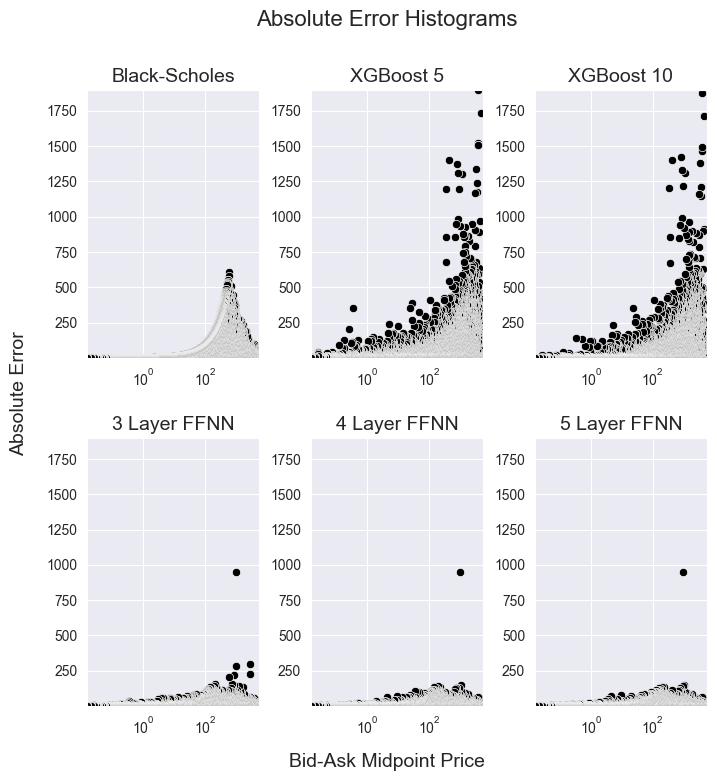
\includegraphics[width=\linewidth]{AE.png}
    \caption{Absolute Error vs. Bid-Ask Midpoint Price}
    \label{fig:AE}
  \end{figure}

\begin{figure}[H]
    \centering
    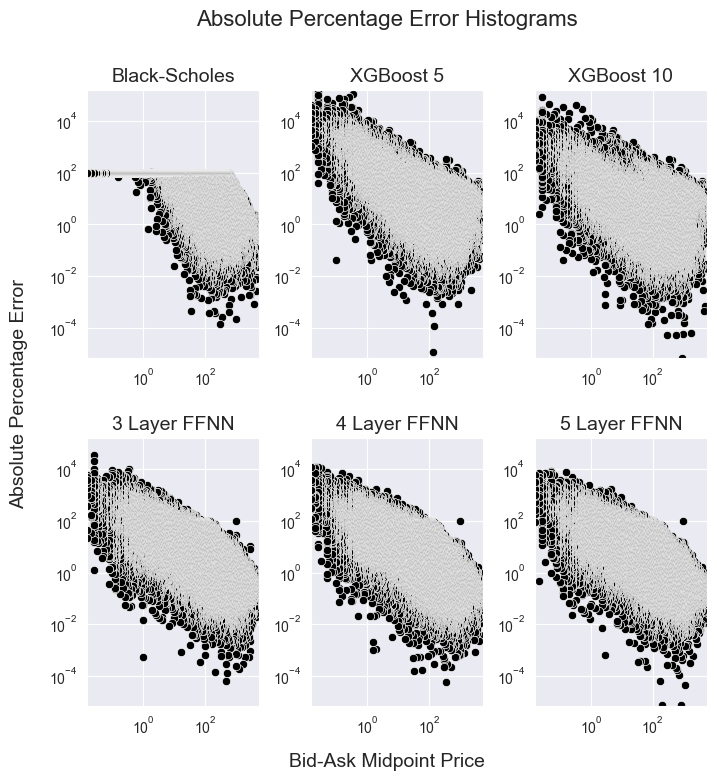
\includegraphics[width=\linewidth]{APE.png}
    \caption{Absolute Percentage Error vs. Bid-Ask Midpoint Price}
    \label{fig:APE}
  \end{figure}

\begin{table}[htbp]
\centering
\caption{Models MAE (100 $<$ Midpoint $<$ 1000)}
\label{table:modelcomparison_mae_filt}
\begin{tabular}{cccc}
\hline
Model & Call & Put & Total \\
\hline
5 Layer FFNN MAE & 7.21 & 7.56 & 7.385 \\
4 Layer FFNN MAE & 7.36 & 7.77 & 7.565 \\
3 Layer FFNN MAE & 8.86 & 9.26 & 9.060 \\
XGBoost 10 MAE & 16.40 & 12.63 & 14.515 \\
XGBoost 5 MAE & 20.01 & 15.95 & 17.980 \\
Black-Scholes MAE & 50.00 & 52.15 & 51.075 \\
\hline
\end{tabular}
\end{table}

\begin{table}[htbp]
\centering
\caption{Models MAPE (100 $<$ Midpoint $<$ 1000)}
\label{table:modelcomparison_mape_filt}
\begin{tabular}{cccc}
\hline
Model & Call & Put & Total \\
\hline
5 Layer FFNN MAPE & 3.44 & 4.18 & 3.810 \\
4 Layer FFNN MAPE & 3.54 & 4.30 & 3.920 \\
3 Layer FFNN MAPE & 4.16 & 5.04 & 4.600 \\
XGBoost 10 MAPE & 5.07 & 4.99 & 5.030 \\
XGBoost 5 MAPE & 6.66 & 6.75 & 6.705 \\
Black-Scholes MAPE & 23.18 & 27.54 & 25.360 \\
\hline
\end{tabular}
\end{table}

\section{Conclusion}
Even though XGBoost is regarded as the industry standard for regression and classification problems, Neural Networks seem to be far superior in estimating options prices than XGBoost. Both machine learning algorithms are able to outperform the Black-Scholes model, but it is clear that Feed-Forward Neural Networks are the superior model. It is also important to note that both the Neural Networks and the Gradient Boosted Decision Tree Models were not given implied volatility as a feature like the Black-Scholes model was, but learned all the necessary features on their own from the other feature variables and the past 20 lags of the underlying securities closing prices. With high volumes of data and computing resources becoming highly available, using machine learning and deep learning methods for options pricing becomes a viable option for pricing securities. It would be also be interesting to compare machine learning and deep learning methodologies with other option pricing methods such as Monte Carlo Simulations or the Binomial Asset Pricing Model in order to see if the Machine Learning models are able to surpass those models as well. Nevertheless, the results of this study seem to be consistent with the results of other related studies in that deep learning methods are able to outperform the Black-Scholes model, and in this case the gold standard in classification and regression problems, the XGBoost algorithm.

\section*{Acknowledgments}

This research project contains components for three graduate level courses at the University of Notre Dame, which are ACMS 80695 - Master's Research Project taught by Prof. Guosheng Fu, CSE 60868 - Neural Networks taught by Prof. Adam Czajka, and ACMS 60890 - Statistical Foundations of Data Science taught by Prof. Xiufan Yu. The Tensorflow Neural Networks were completed for CSE 60868, the XGBoost models were completed for ACMS 60890, and the research methodologies and big data applications in google cloud were performed as part of the ACMS 80695 project. A special thanks is given to all these professors for their teaching and support during the Spring Semester of 2023.


\begin{thebibliography}{99}

\bibitem{ke2019option}
Alexander Ke and Andrew Yang.
\newblock Option Pricing with Deep Learning.
\newblock {\em CS230: Deep Learning, Fall 2019, Stanford University, CA}, 2019.

\bibitem{malliaris1993beating}
M.~Malliaris and L.~Salchenberger.
\newblock Beating the best: a neural network challenges the Black-Scholes formula.
\newblock In {\em Proceedings of 9th IEEE Conference on Artificial Intelligence for Applications}, pages 445--449. IEEE, 1993.

\bibitem{leRoux2001}
L. J. le Roux and G. S. du Toit.
\newblock Emulating the Black \& Scholes model with a neural network.
\newblock {\em Southern African Business Review}, 5(1):54--57, 2001.

\bibitem{mitra2012option}
S.~K. Mitra.
\newblock An option pricing model that combines neural network approach and Black-Scholes formula.
\newblock {\em Global Journal of Computer Science and Technology}, 12(4):1--9, 2012.

\bibitem{can2014nonparametric}
M. Can and S. Fadda.
\newblock A nonparametric approach to pricing options using learning networks.
\newblock {\em Southeast Europe Journal of Soft Computing}, 3(1):, 2014.

\bibitem{ruf2020neural}
Johannes Ruf and Weiguan Wang.
\newblock Neural networks for option pricing and hedging: a literature review.
\newblock {\em Journal of Computational Finance}, 24(4):91--120, 2020.
\newblock arXiv:1911.05620.

\bibitem{optionmetrics}
Wharton Research Data Services.
\newblock IvyDB US by OptionMetrics (optionm\_all).
\newblock \url{https://wrds.wharton.upenn.edu/}, 2022.
\newblock Accessed: 2023-04-25.

\end{thebibliography}



\onecolumn % switch to one column

\appendix
\section{\label{sec:appendix}Appendix}

\begin{table}[htbp]
\centering
\caption{Summary Statistics for Financial Data}
\label{table:financialdata}
\begin{tabular}{ccccccc}
\hline
Statistic & Midpoint & Strike Price & Imp. Volatility & Zero Coupon Rate & Div. Yield & Time (years)\\
\hline
count & \num{10750890} & \num{10750890} & \num{10750890} & \num{10750890} & \num{10750890} & \num{10750890}\\
mean & \num{128.88} & \num{1369.92} & \num{0.51} & \num{2.90} & \num{2.36} & \num{0.59}\\
std & \num{306.93} & \num{2406.36} & \num{0.44} & \num{1.997617} & \num{2.04} & \num{0.53}\\
min & \num{0.015} & \num{5} & \num{0.0112} & \num{0.2935} & \num{0.000107} & \num{0.00274}\\
25\% & \num{6.5} & \num{275} & \num{0.2354} & \num{1.29} & \num{1.27} & \num{0.2163}\\
50\% & \num{32} & \num{620} & \num{0.3669} & \num{2.21} & \num{1.88} & \num{0.5202}\\
75\% & \num{112.1} & \num{1495} & \num{0.6167} & \num{4.58} & \num{2.54} & \num{0.7392}\\
max & \num{13267} & \num{21500} & \num{2.99999} & \num{7.63} & \num{147.35} & \num{4.7967}\\
\hline
\end{tabular}
\end{table}

\begin{multicols}{2}
  \begin{figure}[H]
    \centering
    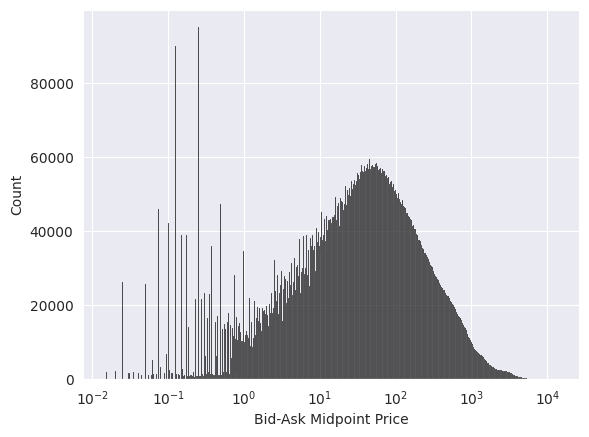
\includegraphics[width=\linewidth]{01_midpoint_dist.png}
    \caption{Distribution of Bid-Ask Midpoint Prices}
    \label{fig:01_midpoint_dist}
  \end{figure}
  
  \begin{figure}[H]
    \centering
    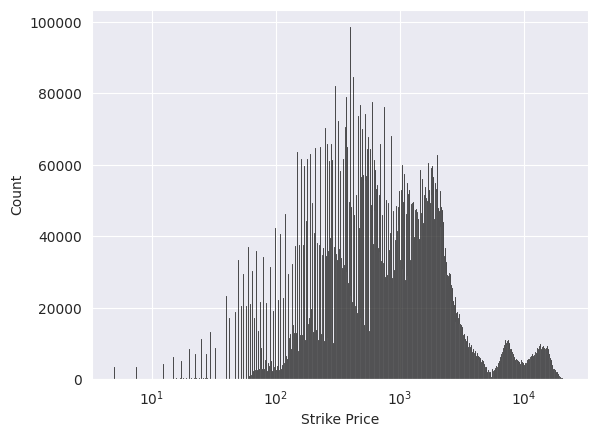
\includegraphics[width=\linewidth]{02_strike_price_dist.png}
    \caption{Distribution of Strike Prices}
    \label{fig:02_strike_price}
  \end{figure}
\end{multicols}

\begin{multicols}{2}
  \begin{figure}[H]
    \centering
    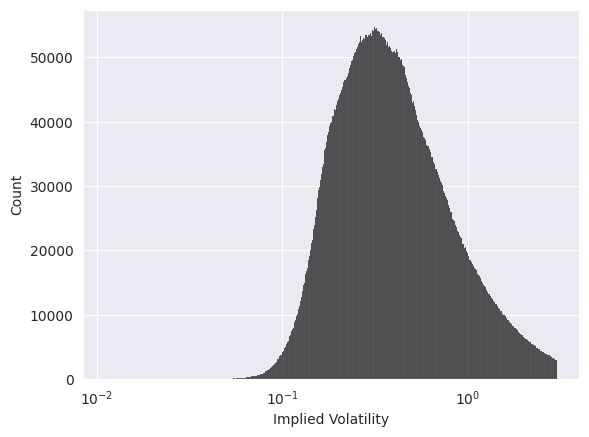
\includegraphics[width=\linewidth]{03_imp_vol_dist.png}
    \caption{Distribution of Implied Volatilities}
    \label{fig:03_imp_vol_dist}
  \end{figure}
  
  \begin{figure}[H]
    \centering
    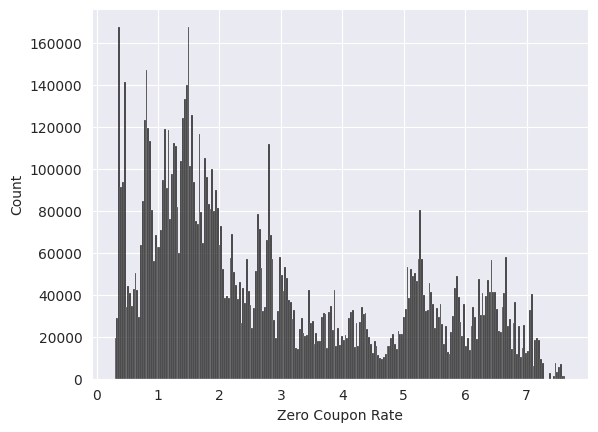
\includegraphics[width=\linewidth]{04_zero_coupon_dist.png}
    \caption{Distribution of Zero Coupon Rates}
    \label{fig:04_zero_coupon_dist}
  \end{figure}
\end{multicols}

\pagebreak

\begin{multicols}{2}
  \begin{figure}[H]
    \centering
    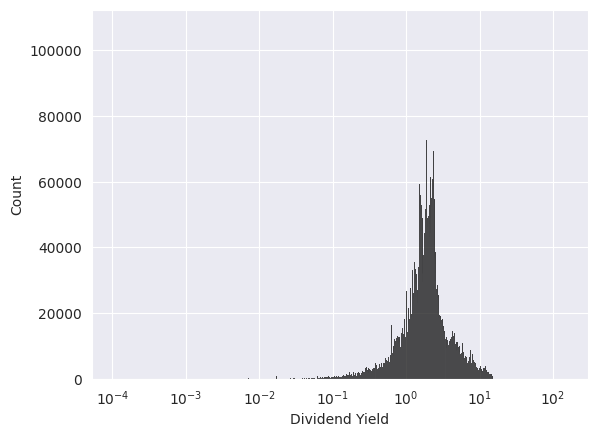
\includegraphics[width=\linewidth]{05_div_yield_dist.png}
    \caption{Distribution of Index Dividend Yields}
    \label{fig:05_div_yield_dist}
  \end{figure}
  
  \begin{figure}[H]
    \centering
    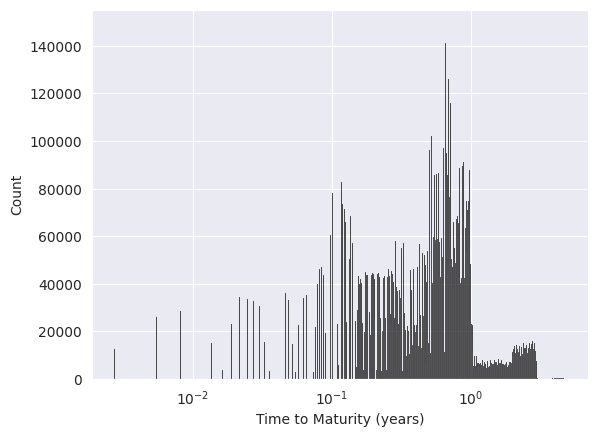
\includegraphics[width=\linewidth]{06_time_dist.png}
    \caption{Distribution of Times to Maturity (years)}
    \label{fig:06_time_dist}
  \end{figure}
\end{multicols}

\begin{multicols}{2}
  \begin{figure}[H]
    \centering
    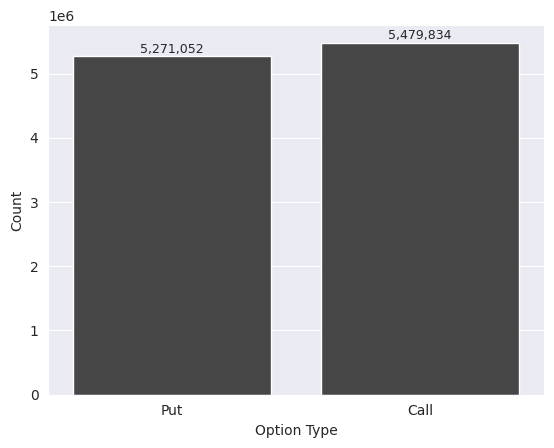
\includegraphics[width=\linewidth]{07_opt_type_dist.png}
    \caption{Distribution of Calls and Puts}
    \label{fig:07_opt_type_dist}
  \end{figure}
\end{multicols}

\end{document}